\documentclass[12pt,a4paper,italian,twoside]{scrbook}
\usepackage[T1]{fontenc}
\usepackage[utf8]{inputenc}
\usepackage{babel}
\usepackage[beramono,pdfspacing,
	eulerchapternumbers,eulermath,floatperchapter]
	{classicthesis} % per uno stile bello
\usepackage{arsclassica}	% per uno stile ancora più bello
%\usepackage{amsmath,amsfonts}
\usepackage{amssymb}
\usepackage{mathtools}
\usepackage{multicol}
\usepackage{array}
\usepackage{pdflscape}
\usepackage[dvipsnames]{xcolor}
\usepackage{colortbl}
\usepackage{graphicx}
\usepackage{wrapfig}	% per didascalie avvolte nel testo
\usepackage{booktabs}
\usepackage{multirow}
%\usepackage{parskip}	% pacchetto per la non indentazione del paragrafo, sconsigliato con scrbook
\usepackage{enumitem}	% per elenchi con label
\usepackage{subcaption}	% più performante rispetto subfigure
\usepackage{geometry}	% cambiare la geometria del decumento
\usepackage{tabularx}	% per stabilire autonomamente la larghezza delle tabelle
\usepackage{rotating}   % per ruotare le scritte all'interno delle tabelle
\usepackage{sidecap}	% per le didascalie laterali
\usepackage{longtable}	% per fare tabelle più lunghe di una pagina
\usepackage{eurosym}    % per mettere il simbolo dell'euro
\usepackage{adjustbox}  % per rendere le tabelle più piccole
\usepackage{verbatim}	% per usare l'ambiente comment
\usepackage[section]{placeins}	% per usare \FloatBarrier; l'opzione lo include in \section{}
\usepackage[swapnames,norules,nouppercase]{frontespizio}%[onlyinclude,nowrite]{frontespizio}	% usato per includere il frontespizio

% licenza
\usepackage{xmpincl}	% permette di includere licenze in formato XMP
\includexmp{files/CC_Attribution-NonCommercial-ShareAlike_4.0_International}	% file della licenza

% bibliografia
\usepackage[autostyle,italian=guillemets]{csquotes}    % per citare con le virgolette giuste
\usepackage[bibstyle=authoryear,citestyle=authoryear-ibid-brack,backend=biber]{
biblatex}       % per la bib
\addbibresource{materiale_iniziale_finale/bibliografia.bib}
%\defbibheading{cartaceo}{\section*{Bibliografia cartacea}}
%\defbibheading{web}{\section*{Sitografia}}

% per scrivere bene le unità di misura
\usepackage{siunitx}
\sisetup{
	output-decimal-marker	=	{.},
	list-final-separator	=	{ e },
	list-pair-separator		=	{ e },
	range-phrase			=	{ a },
	per-mode				=	symbol,
    sticky-per 				=	true,
    detect-all				=	true,
}
\DeclareSIUnit\anni{anni}
\DeclareSIUnit\anno{anno}
\DeclareSIUnit\minuti{minuti}
\DeclareSIUnit\minuto{minuto}
\DeclareSIUnit\ore{ore}
\DeclareSIUnit\ora{ora}
\DeclareSIUnit\none{-}
\DeclareSIUnit\e{\euro}

% per personalizzare le caption
\begin{comment}
\usepackage{caption}
\captionsetup{
	labelformat=simple, % simple senza parentesi, parens con le parentesi
	font={it},
	labelfont=bf,
	justification=centerlast
}
\end{comment}

% serie di pacchetti per la stesura con Latex di grafici e disegni
\usepackage{tikz}
\usepackage{pgfplots}	% pacchetto per grafici
\pgfplotsset{compat=newest}	% ultima versione
\SendSettingsToPgf
\usepgfplotslibrary{fillbetween}	% per riempire di colore i grafici
\usepgfplotslibrary{dateplot}	% per usare date come numeri
\usepgfplotslibrary{statistics}	% per fare boxplot
\usepgfplotslibrary{groupplots}	% per fare grafici a gruppi
\usepgfplotslibrary{units}	% to add units easily to axis
\usepgfplotslibrary{colormaps}	% to create colormaps
\pgfdeclarehorizontalshading{visiblelight}{50bp}{
color(0.00000000000000bp)=(violet);
color(8.33333333333333bp)=(blue);
color(16.66666666666670bp)=(cyan);
color(25.00000000000000bp)=(green);
color(33.33333333333330bp)=(yellow);
color(41.66666666666670bp)=(orange);
color(50.00000000000000bp)=(red)
}%
\usepgfplotslibrary{external}	% per creare pdf esterni dei grafici
\tikzexternalize

% per riferimenti
\usepackage{hyperref}
\hypersetup{
	colorlinks	=	true,	% attiva il colore per i link, altrimenti sono inscatolati
	%linkcolor	=	black,	% il colore dei link è nero
	pdftitle	=	Tesi: Dinamiche vegetazionali nel fiume Tagliamento,
	pdfauthor	=	Castellani Robin,
	%hidelinks,
}
\usepackage{varioref}	% per riferimenti con pagine
\usepackage{cleveref}	% per riferimenti intelligenti

%\crefname{equation}{equazione}{equazioni}

% glossario
\usepackage[translate=babel,nonumberlist]{glossaries}
\makeglossaries
\loadglsentries{materiale_iniziale_finale/voci-glossario}

\newcommand{\AST}{ASTER}
\newcommand{\Se}{Sentinel2}
\newcommand{\Pl}{Pleiades}
\newcommand{\WV}{WorldView2}

\hyphenation{NDVI}


\begin{document}
%**********************************************************
%**********************************************************
\frontmatter
%----------------------------------------------------------
\begin{Preambolo*}
	\usepackage {fontspec} % per nuovi font, compila con XeLaTeX
	\newfontfamily \frntitle {Quadrat Serial} % per logo università
	\setmainfont {Tahoma} % per tutto il resto
	\renewcommand{\frontinstitutionfont}{%
		\fontsize{18}{17}\selectfont}
	\renewcommand{\frontdivisionfont}{%
		\fontsize{18}{16}\selectfont}
	\renewcommand{\fronttitlefont}{%
		\fontsize{18}{16}\selectfont}
	\renewcommand{\frontfixednamesfont}{%
		\fontsize{14}{16}\selectfont}
	\renewcommand{\frontnamesfont}{%
		\fontsize{14}{16}\selectfont}
	\renewcommand{\frontfootfont}{%
		\fontsize{14}{16}\selectfont}
	\Margini {2cm}{5.9cm}{2cm}{1.9cm}
	\NCandidato{Laureando}
	\Punteggiatura % elimina i : dopo Relatore e Laureando
\end{Preambolo*}
%
\begin{frontespizio}
	\Istituzione {{\frntitle UNIVERSIT\`{A} DEGLI STUDI DI TRENTO}}
	\Logo [2.65cm]{files/logo_UniTN.jpg}
	\Dipartimento {Ingegneria Civile Ambientale Meccanica}
	\Corso {\\Ingegneria per l'Ambiente e il Territorio}
	\Titolo {
		Dinamiche della vegetazione riparia nel fiume Tagliamento:
		\\
		traiettorie evolutive e relazioni piene - vegetazione
	}
	\Candidato {Robin Castellani}
	\Relatore {Prof. Walter Bertoldi}
	\Annoaccademico {2017-2018}
\end{frontespizio}


%----------------------------------------------------------
\tableofcontents
\listoffigures
\listoftables
%----------------------------------------------------------
\chapter{Prefazione}
%\begin{abstract}
La presente tesi mira a studiare come cambia la vegetazione nel fiume braided Tagliamento in risposta all'idrologia. 
L'obiettivo principale è quello di ricercare una relazione tra i livelli del pelo libero registrati da alcuni idrometri e la vegetazione erosa, tra i livelli e la quantità di legname che si ritrova in alveo.

Si analizzano immagini satellitari e ortofoto al fine di distinguere la parte vegetata dell'alveo e il legname presente.
Con i dati di piovosità media mensile e di temperatura media mensile si cercano correlazioni con l'espansione della vegetazione che si osserva negli anni.
Dalla quantificazione dell'erosione della vegetazione dovuta alle piene, della quantità di legno in alveo e di un tasso di crescita della vegetazione si tenta di costruire un bilancio di materia vegetale a scala di evento di piena.
Inoltre si trovano valori soglia per l'erosione della vegetazione.
%\end{abstract}

%----------------------------------------------------------



%**********************************************************
%**********************************************************
\mainmatter
\chapter{Inizio}
\section{Introduzione}
La presente tesi mira a studiare come cambia la vegetazione nel fiume Tagliamento in risposta al regime idrologico (successione di magre, piene \emph{bankfull}, \emph{flood pulses}).
L'obiettivo principale è quello di ricercare una relazione che leghi i livelli del pelo libero dell'acqua registrati da un idrometro con la quantità di vegetazione erosa in seguito ad una piena, o che leghi i livelli con la quantità di legname che si ritrova in alveo dopo eventi di piena.
In via previsionale si cerca di rispondere all'esigenza di stimare in anticipo gli effetti sulle isole che può avere una piena in questo fiume.
\\
Inoltre si trovano traiettorie evolutive per quanto riguarda la larghezza e la percentuale di isole rispetto all'alveo attivo, anche confrontando i dati ottenuti per un tratto di qualche chilometro con alcuni risultati da letteratura; si ottengono relazioni tra la forza della corrente (\emph{stream power}) e la quantità massima di isole presenti.
%Inoltre si trovano valori soglia del livello del pelo libero per l'erosione della vegetazione.
%\\
%Dalla quantificazione dell'erosione della vegetazione dovuta alle piene, della quantità di legno in alveo e di un tasso di crescita della vegetazione si tenta di costruire un bilancio di materia vegetale a scala di evento di piena.

Si analizzano immagini satellitari e ortofoto al fine di distinguere la parte dell'alveo ricoperta da vegetazione (\vref{fig:esempio-isola-1}) e gli elementi legnosi (tronchi e accumuli di legno, \vref{fig:esempio-accumulo-1}).

\begin{figure}
	\centering
	\begin{subfigure}[b]{0.37\textwidth}
		\includegraphics[width=\textwidth]{files/esempio_isola_sat_1.jpg}
		\caption{immagine da Google Earth di un isola in alveo.}
		\label{fig:esempio-isola-sat-1}
	\end{subfigure}
	\quad
	\begin{subfigure}[b]{0.57\textwidth}
		\includegraphics[width=\textwidth]{files/esempio_isola_1.jpg}
		\caption{foto di un isola molto vegetata presente nell'alveo del fiume.
		Foto dell'autore.}
		\label{fig:esempio-isola-1}
	\end{subfigure}
	\caption[immagine e foto di isole fluviali]{immagine e foto di isole fluviali; si noti la forte presenza di salici (\emph{Salix spp.}) e di pioppi (\emph{Populus spp.}); il luogo della foto è prossimo a quello dell'immagine.}
\end{figure}

\begin{figure}
	\centering
	\begin{subfigure}[b]{0.52\textwidth}
		\includegraphics[width=\textwidth]{files/esempio_accumulo_sat_1.jpg}
		\caption{immagine da Google Earth di accumuli di legno e tronchi in alveo (in marrone chiaro).}
		\label{fig:esempio-accumulo-sat-1}
	\end{subfigure}
	\quad
	\begin{subfigure}[b]{0.44\textwidth}
		\includegraphics[width=\textwidth]{files/esempio_accumulo_1.jpg}
		\caption{foto di un accumulo di tronchi sopra una pianta di salice.
		Foto dell'autore.}
		\label{fig:esempio-accumulo-1}
	\end{subfigure}
	\caption[immagine e foto di accumuli legnosi]{immagine e foto di accumuli legnosi. Il luogo della foto non corrisponde a quello dell'immagine.}
\end{figure}


\section{Inquadramento dell'area di studio}
Il Fiume Tagliamento, situato nel Nord-Est italiano, è uno dei pochi fiumi alpini allo stato quasi naturale. 
Gli interventi effettuati sono arginature, derivazioni, pennelli, estrazione di ghiaia sia in tratti posti a monte che altri posti a valle; la loro entità è comunque tanto limitata da poter parlare di “contesto non gestito”.
\\
Il bacino idrografico del Tagliamento, ampio circa~\SI{2900}{\kilo\m\tothe{2}}, si estende tra le province di Udine, Pordenone e Venezia.
Il suo corso di circa~\SI{170}{\kilo\m} presenta morfologia intrecciata (\emph{braided}) nelle parti montane e planiziali con tratti larghi diverse centinaia di metri, se non più di \SI{1}{\kilo\m};
verso valle il fiume si restringe assumendo prima una forma transizionale monocursale con larghezza sui \SIrange[range-phrase={-}]{300}{200}{\m} nei pressi di Madrisio;
infine meandriforme a Latisana (larghezza intorno ai \SI{100}{\m}) fino alla foce, situata tra Bibione e Lignano.
\\
Insieme alla variazione della morfologia del fiume si assiste ad un cambiamento nella granulometria: mentre la ghiaia predomina nella parte intrecciata ($d_{50} = \SI{4}{\centi\m}$ \squarecites{Bertoldi:2010-d50}{Sitzia:2016-d50}), a partire dal tratto meandriforme si trova solo sabbia sul fondo.
Questo mutamento di materiale trasportato riflette la riduzione della pendenza che si osserva dal tratto transizionale monocursale e che giustifica il passaggio da fiume “in ghiaia” a fiume “in sabbia”.
\\
Il regime delle precipitazioni consiste di circa \SI{2000}{\mm} all'anno in media con forti variazioni locali; i minimi di precipitazione si registrano durante l'inverno, mentre i massimi in primavera e in autunno. Si assiste anche ad eventi di breve durata e particolarmente intensi.
Il regime fluviale che ne risulta è di tipo \emph{flashy} pluvio-nivale con piene brevi ed intense così come piene di diversi giorni di durata.

Il tratto studiato è quello intrecciato multicanale compreso tra Tolmezzo e Madrisio (\vref{fig:overview,fig:overview-sat}). 

In questo tratto nei pressi del paese di Pinzano è presente una stretta causata dall'affioramento di strati rocciosi che riduce la larghezza da diverse centinaia di metri a poco più di \SI{100}{\m}.
Questo restringimento assieme all'innalzamento dello strato di roccia che si trova sotto il letto del fiume induce l'acqua presente nella falda in alveo a risalire: si assiste al fenomeno dell'\emph{upwelling}. 
Similmente, a valle della stretta dove l'alveo non è più confinato e il letto roccioso sprofonda nel sottosuolo, l'acqua torna ad infiltrarsi nella ghiaia che forma il letto (\emph{downwelling}) fino a portare il fiume in condizioni di secca in certi tratti quando non ci sono piene.
\\
L'\emph{upwelling} e il \emph{downwelling} sono fenomeni rilevanti durante i periodi di magra: certi tratti a valle della stretta di Pinzano possono essere in condizioni di secca, privi completamente di acqua, la quale scorre tutta nel sottosuolo e riemerge quando la morfologia fluviale diventa transizionale vicino al ponte di Madrisio.
Durante le piene questi fenomeni sono invece irrilevanti: l'acqua che emerge o che si infiltra contribuisce minimamente alla portata fluente.

Nel tratto di studio vi sono diversi affluenti; vengono qui elencati da monte (Tolmezzo) fino a valle (Madrisio):
%
\begin{itemize}
	\item poco a valle di Tolmezzo c'è il Fella in sinistra idrografica (\SI{706}{\kilo\m\tothe{2}});
	\item all'altezza del paese di Venzone, in sinistra idrografica, sfocia il torrente Venzonassa (\SI{39}{\kilo\m\tothe{2}});
	\item qualche chilometro a monte del paese di Cornino in destra idrografica c'è il Leale (\SI{100}{\kilo\m\tothe{2}}), le cui acque riempiono i canali incisi del Tagliamento che in magra sono quasi secchi;
	\item in corrispondenza dell'isola di Cornino in sinistra idrografica il Ledra (\SI{75}{\kilo\m\tothe{2}}) riporta nel corso del Tagliamento le acque che si sono infiltrate nella piana di Osoppo;
	\item immediatamente a monte della stretta di Pinzano in destra idrografica si getta l'Arzino (\SI{123}{\kilo\m\tothe{2}});
	\item infine, una decina di chilometri più a valle della stretta in destra idrografica si incontra il Cosa (\SI{160}{\kilo\m\tothe{2}}).
\end{itemize}
%
Il contributo di questi affluenti in termini di portata non è trascurabile; tuttavia è raro che eventi di piena abbiano luogo contemporaneamente in tutti i sottobacini tanto da incrementare sensibilmente il livello d'acqua nel Tagliamento a valle degli affluenti durante una piena.
Si ritiene pertanto che conoscere il livello d'acqua in un punto del Tagliamento sia sufficientemente rappresentativo per descrivere l'entità di una piena in tutto il tratto di studio; inoltre si assume che la portata fluente sia proporzionale all'area drenante in ogni sezione del fiume.
%TODO immagine degli affluenti

%
\begin{figure}
	\centering
	\includegraphics[width=\textwidth]{files/overview.jpeg}
	\caption[inquadramento dell'area di studio]
		{inquadramento dell'area di studio (poligono nero); a sinistra è mostrata l'Italia settentrionale (in alto) e un ingrandimento delle province e degli estremi dell'area di studio (in basso); a destra si vede il bacino idrografico del Tagliamento e di altri fiumi nelle vicinanze (in blu), il reticolo idrografico (in azzurro) e la linea di costa (in verde acqua).}
	\label{fig:overview}
\end{figure}
%
\begin{figure}
	\centering
	\includegraphics[width=\textwidth]{files/overview_tratto_sat.jpeg}
	\caption[inquadramento dell'area di studio]{inquadramento dell'area di studio (contornata in giallo).}
	\label{fig:overview-sat}
\end{figure}



\section{Stato dell'arte e valore aggiunto del presente lavoro}
In letteratura sono presenti numerosi lavori focalizzati su un tratto di circa~\SI{12}{\kilo\m} di lunghezza a monte della stretta di Pinzano; solitamente questi hanno utilizzato immagini ad alta risoluzione provenienti da voli aerei, le quali hanno una bassa risoluzione temporale (meno di una decina di immagini su un periodo di studio di diversi decenni).
\\
Le analisi svolte sono simili a quelle che questa tesi si propone di presentare: ricerca di una relazione tra isole erose e portata \squarecite{Surian:2015}, osservazione dell'evoluzione delle isole e della larghezza \squarecites{Surian:2015}{Bertoldi:2011-ASTER}{Zanoni:2008}.
\\
Le immagini satellitari \AST{} o LandSat~TM sono state utilizzate per gli scopi simili a quelli della presente tesi \squarecites{Bertoldi:2011-ASTER}{Henshaw:2013-LandSat}.
\\
Sono stati formulati diversi modelli concettuali sulle dinamiche vegetazionali nei fiumi, in particolare nel Tagliamento \squarecites{Gurnell:2001-island-formation}{Gurnell:2014-plants-eng}.

% i risultati di questi lavori attinenti al tema della tesi sono:
% a seguito di un progressivo restringimento esperito nella seconda metà del '900, nel primo decennio del 2000 il Tagliamento si è allargato

Il presente lavoro mira a :
\begin{itemize}
	\item utilizzare un maggior numero di immagini in un periodo di studio più breve, avvalendosi dei prodotti sia delle più recenti missioni spaziali sia di quelle relativamente più datate, e in un tratto di fiume più esteso; in tal maniera possono essere analizzati più fenomeni in maggior dettaglio;
	\item utilizzare ed estendere le metodologie, e di conseguenza anche i risultati, applicabili nello sfruttamento delle immagini satellitari;
	\item attraverso osservazioni e relazioni formalizzare modelli concettuali precedentemente elaborati;
	\item utilizzare dati provenienti da rilievi LiDAR per calcolare la \emph{stream power};
	\item ottenere delle relazioni più solide grazie alla maggior quantità di dati disponibili;
	\item aggiungere nuove osservazioni a quelle effettuate in precedenza;
	\item mostrare che è possibile effettuare un monitoraggio delle dinamiche fluviali quasi in tempo reale. 
\end{itemize}



\section{Convenzioni}
Le seguenti convenzioni saranno utilizzate nella presente tesi:
\begin{description}
	\item[Mappe] riportate secondo WGS84/UTM~33N (EPSG:~32633);
	\item[Direzione della corrente] riportata con una freccia blu nelle immagini;
	\item[Formato delle date] AAAA-MM-GG;
	\item[Citazioni] sono nel formato Autore/i-Anno, racchiuse tra parentesi quadre;
	\item[Web link] sono riportati in note a piè pagina;
	\item[Termini in lingua straniera] sono in corsivo;
	\item[Glossario] presente nel materiale finale.
	%
\end{description}




\section{Lo strumento principale: la radiazione elettromagnetica}
Gli strumenti di acquisizione di immagini aeree e satellitari sono sensibili a determinate lunghezze d'onda della radiazione elettromagnetica (\vref{graph:el-mag-radiation}), cioè sono in grado di registrarne solo alcune porzioni (bande).
L'occhio umano può distinguere solo le bande del visibile, mentre i sensori artificiali possono acquisire altre bande della radiazione.
%
\begin{figure}
	\centering
	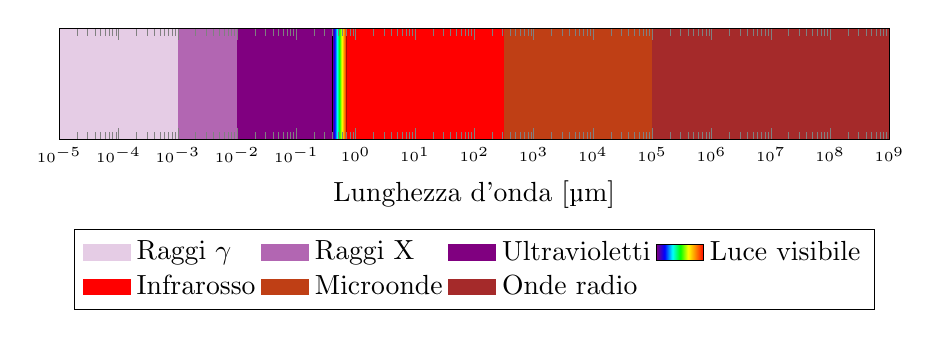
\begin{tikzpicture}[fill between/on layer={axis grid}]
	\begin{axis}[
		xlabel={Lunghezza d'onda},
		xticklabel style = {font=\tiny,yshift=0.2ex},
		xmin=10^-5,
		xmax=10^9,
		x unit=\si{\micro\meter},
		xmode=log,
		ymin=0,
		ymax=1,
		height=3cm,
		width=\textwidth,%12.2cm,
		yticklabels={},
		ytick=\empty,
		legend cell align=left,
		legend style={
			at={(0.5,-0.8)},%(0.85,-0.77)},
			anchor=north,
			legend columns=4,
			}
	]
	\addplot[draw=none, name path=start, forget plot] coordinates{(10^-5,0)(10^-5,1)};
	\addplot[draw=none, name path=gamma, forget plot] coordinates{(10^-3,0)(10^-3,1)};
	\addplot[draw=none, name path=xrays, forget plot] coordinates{(10^-2,0)(10^-2,1)};
	\addplot[draw=none, name path=uv, forget plot] coordinates{(0.4,0)(0.4,1)};
	\addplot[draw=none, name path=visible, forget plot] coordinates{(0.7,0)(0.7,1)};
	\addplot[draw=none, name path=ir, forget plot] coordinates{(10^2.5,0)(10^2.5,1)};
	\addplot[draw=none, name path=microwave, forget plot] coordinates{(10^5,0)(10^5,1)};
	\addplot[draw=none, name path=radiowave, forget plot] coordinates{(10^9,0)(10^9,1)};
	\addplot[violet!20, area legend] fill between[of=start and gamma];
	\addlegendentry{Raggi $\gamma$}
	\addplot[violet!60, area legend] fill between[of=gamma and xrays];
	\addlegendentry{Raggi X}
	\addplot[violet, area legend] fill between[of=xrays and uv];
	\addlegendentry{Ultravioletti}
	\addplot[shading=visiblelight, area legend] fill between[of=uv and visible];
	\addlegendentry{Luce visibile}
	\addplot[red, area legend] fill between[of=visible and ir];
	\addlegendentry{Infrarosso}
	\addplot[Bittersweet, area legend] fill between[of=ir and microwave];
	\addlegendentry{Microonde}
	\addplot[Brown, area legend] fill between[of=microwave and radiowave];
	\addlegendentry{Onde radio}
	\end{axis}
\end{tikzpicture}

	\caption{radiazione elettromagnetica con le sue lunghezze d'onda.}
	\label{graph:el-mag-radiation}
\end{figure}
%
\\
Le immagini nel visibile sono solitamente suddivise nelle bande del Rosso, Verde e Blu (\emph{Red}, \emph{Green}, \emph{Blue}, R-G-B); ognuna indica la quantità di colore presente; la combinazione di queste quantità di colore restituisce l'immagine a colori.
\\
Per poter osservare immagini con bande diverse dal visibile si sostituisce una o più bande R-G-B con le bande in questione.
Ad esempio, è possibile sostituire la banda del Rosso con quella dell'Infrarosso (IR): la quantità di colore del Rosso sarà rimpiazzata dalla quantità di colore dell'Infrarosso.
Il risultato sarà un'immagine riconoscibile dall'occhio umano, ma in falsi colori (\vref{fig:confronto-bande-intro}).
%
\begin{figure}
	\centering
	\includegraphics[width=\textwidth]{files/confronto_bande_intro.jpeg}
	\caption[confronto immagini R-G-B e IR-R-G]{confronto di un'immagine in veri colori (R-G-B, a sinistra) con una in falsi colori (IR-G-B, a destra); quest'ultima evidenza la presenza di vegetazione viva rispetto alla ghiaia in alveo e all'acqua nei canali.}
	\label{fig:confronto-bande-intro}
\end{figure}
%
\\
Questo procedimento serve per distinguere più facilmente degli elementi e degli oggetti presenti nelle immagini; per esempio la vegetazione viva riflette particolarmente la banda dell'Infrarosso più vicina al Rosso.



\section{Materiali}
% materiali
\paragraph{Immagini aeree e satellitari}
Sono state considerate le bande del \emph{Near-InfraRed}~(NIR) e del \emph{Red}~(R) nelle immagini satellitari multibande provenienti dalle seguenti missioni:
%
\begin{itemize}
	\item satellite Terra, sensore \AST{} Livello~1T (ottenuti in data~21~luglio~2018 e~30~settembre~2018 \squarecite{data:ASTER});  
		\\
		NIR (Banda~3N)~\SIrange[range-phrase={-}]{0.78}{0.86}{\nano\m}, R (Banda~2)~\SIrange[range-phrase={-}]{0.63}{0.69}{\micro\m};
	\item costellazione \Pl{} (\href{https://pleiades.cnes.fr/en/PLEIADES/index.htm}{Centre National d'Etudes Spatiales}\footnote{\texttt{https://pleiades.cnes.fr/en/PLEIADES/index.htm}}), immagini acquistate dall'Università degli Studi di Trento; 
		\\
		NIR~\SIrange[range-phrase={-}]{0.74}{0.94}{\micro\m}, R~\SIrange[range-phrase={-}]{0.59}{0.71}{\micro\m};
	\item satellite \Se{}A-B, sensore~MSI Livello~1C (ottenuti in data 21~luglio 2018 e~21~novembre~2018 tramite il \href{http://scihub.copernicus.eu/}{Copernicus Open Access Hub}\footnote{\texttt{http://scihub.copernicus.eu/}});
		\\
		NIR (Banda~8)~\SIrange[range-phrase={-}]{0.763}{0.908}{\micro\m}, R (Banda~4)~\SIrange[range-phrase={-}]{0.645}{0.683}{\micro\m};
	\item satellite \WV{} (\href{satimagingcorp.s3.amazonaws.com/site/pdf/WV1\_{}WV2\_{}SpectralResponse.pdf}{DigitalGlobe}\footnote{\texttt{satimagingcorp.s3.amazonaws.com/site/pdf/WV1\_{}WV2\_{}SpectralResponse.pdf}}), immagini acquistate dall'Università degli Studi di Trento;
		\\
		NIR (Banda~MS1)~\SIrange[range-phrase={-}]{0.770}{0.895}{\micro\m}, R (Banda~MS2)~\SIrange[range-phrase={-}]{0.630}{0.690}{\micro\m}.
\end{itemize}
%

Le ortofoto dell'estate~2011 provengono dal \href{http://www.pcn.minambiente.it/mattm/}{Portale Cartografico Nazionale del Ministero dell'Ambiente e della tutela del territorio e del mare}\footnote{\texttt{http://www.pcn.minambiente.it/mattm/}};
le ortofoto del~2013 sono state ottenute da volo \href{http://www.cgrspa.com/}{CGR}\footnote{\texttt{http://www.cgrspa.com/}} su commissione; 
le ortofoto del~2017 sono state ottenute da \href{https://www.google.com/earth/}{Google Earth}\footnote{\texttt{https://www.google.com/earth/}}.

Assieme alla ortofoto del~2013 è stato effettuato un rilievo LiDAR, grazie al quale sono a disposizione un DEM (\emph{Digital Elevation Model}) e un CSM (\emph{Canopy Surface Model}): il primo consiste di una mappa con le quote del suolo; il secondo è una mappa di altezza della vegetazione.

Il DEM del~2009 proviene dal \href{http://irdat.regione.fvg.it/CTRN/ricerca-cartografia/}{Portale Cartografico della regione autonoma Friuli Venezia Giulia}\footnote{\texttt{http://irdat.regione.fvg.it/CTRN/ricerca-cartografia/}}.

È bene evidenziare che le mappe non hanno tutte la medesima estensione e una piccola parte non comprende tutto il tratto oggetto di studio.
Ciò limita minimamente le analisi che è possibile fare.
\\
La risoluzione temporale, inferiore ad~\SI{1}{\anno} con \num{25} immagini per un periodo di studio di quasi \SI{19}{\anni}, è sufficiente per interpretare i processi che hanno luogo nel Tagliamento; la risoluzione spaziale varia da~\SIrange[range-phrase={ a }]{15}{0.5}{\m}, adeguata per poter distinguere correttamente le caratteristiche del fiume (limite dell'alveo attivo, isole, canali nella \emph{floodplain}, canali attivi, \ldots).

\paragraph{Dati idrometrici}
I dati idrometrici orari o semi-orari dal 2000-01-01 al 2018-10-14 presso l'idrometro di Villuzza (\SI{46.181}{\degree}N, \SI{12.958}{\degree}E, quota~\SI{240}{\m}~s.l.m.m., corrispondente al ponte di Pinzano) sono stati forniti dalla \href{http://www.protezionecivile.fvg.it/it/rete-idrometeorologica}{rete idrometeorologica della Protezione Civile della Regione Autonoma Friuli Venezia Giulia}\footnote{\texttt{http://www.protezionecivile.fvg.it/it/rete-idrometeorologica}}.
Questi dati consistono dell'altezza del pelo libero dell'acqua rispetto ad un livello di riferimento locale dell'idrometro.
La dinamica della morfologia del fondo del fiume non permette di ottenere una scala di deflusso (delle portate) generalmente valida; ciò comunque non costituisce un limite.

I grafici in \vref{graph:livelli-orto-sat} mostrano rispettivamente la media giornaliera dei livelli idrometrici e le date di cui si dispongono ortofoto e immagini satellitari (\AST{}, \Pl{}, \Se{}, Google~Earth, \WV{}). 
Nel secondo grafico sono riportati solamente i livelli medi giornalieri maggiori di~\SI{2}{\m} in quanto livelli superiori a tale soglia iniziano ad avere effetti di disturbo sulla vegetazione \squarecite{Bertoldi:2009-2m}.
La \vref{tab:date-orto-sat} mostra le date e la dimensione delle celle delle immagini utilizzate nell'analisi.
%%
\begin{figure}[p]
	\centering
	\begin{tikzpicture}
	\begin{axis}[
		width = \textwidth,
		date coordinates in = x,
		xticklabel = {\year-\month-\day},
		xticklabel style = {
			rotate = 90,
			anchor = near xticklabel
		},
		]
		\addplot table [x=data, y=media-gg] {graphics/data/Dati_Villuzza.csv};
	\end{axis}
\end{tikzpicture}
	\tikzsetnextfilename{livelli_2m+imm}
\begin{tikzpicture}
	\begin{axis}[
		width = \textwidth,
		height = 0.5\textwidth,
		date coordinates in = x,
		date ZERO = 2000-01-01,
		xticklabel = {$\year$},
		xticklabel style = {
			rotate = 80,
			anchor = near xticklabel
		},
		xtick distance = 732,
		enlarge x limits = 0.05,
		enlarge y limits = 0.01,
		%ymax = 3.7,
		ymin = 1.45,
		ylabel = {Livello idrometrico \si{[\m]}},
		grid = major,
		]
		\addplot 
			[fill = red, mark = diamond*, mark size = 4pt,]
			coordinates {(2000-09-17, 1.5)};
		\addplot 
			[fill = red, mark = diamond*, mark size = 4pt,]
			coordinates {(2001-06-07, 1.5)};
		\addplot
        	[fill = red, mark = diamond*, mark size = 4pt,]
        	coordinates {(2002-05-18, 1.5)};
		\addplot
        	[fill = red, mark = diamond*, mark size = 4pt,]
        	coordinates {(2002-06-12, 1.5)};
		\addplot
        	[fill = red, mark = diamond*, mark size = 4pt,]
        	coordinates {(2003-06-22, 1.5)};
		\addplot
        	[fill = red, mark = diamond*, mark size = 4pt,]
        	coordinates {(2004-10-14, 1.5)};
		\addplot
        	[fill = green, mark = diamond*, mark size = 4pt,]
        	coordinates {(2005-05-01, 1.5)};
		\addplot
        	[fill = red, mark = diamond*, mark size = 4pt,]
        	coordinates {(2005-08-30, 1.5)};
		\addplot
        	[fill = red, mark = diamond*, mark size = 4pt,]
        	coordinates {(2006-07-16, 1.5)};
		\addplot
        	[fill = red, mark = diamond*, mark size = 4pt,]
        	coordinates {(2007-09-21, 1.5)};
		\addplot
        	[fill = red, mark = diamond*, mark size = 4pt,]
        	coordinates {(2008-07-05, 1.5)};
		\addplot
        	[fill = red, mark = diamond*, mark size = 4pt,]
        	coordinates {(2009-07-08, 1.5)};
		\addplot
        	[fill = green, mark = diamond*, mark size = 4pt,]
        	coordinates {(2010-08-01, 1.5)};
		\addplot
        	[fill = red, mark = diamond*, mark size = 4pt,]
        	coordinates {(2010-09-29, 1.5)};
		\addplot
        	[fill = green, mark = diamond*, mark size = 4pt,]
        	coordinates {(2011-07-01, 1.5)};
		\addplot
        	[fill = red, mark = diamond*, mark size = 4pt,]
        	coordinates {(2011-10-02, 1.5)};
		\addplot
        	[fill = red, mark = diamond*, mark size = 4pt,]
        	coordinates {(2012-08-01, 1.5)};
		\addplot
        	[fill = red, mark = diamond*, mark size = 4pt,]
        	coordinates {(2013-09-05, 1.5)};
		\addplot
        	[fill = green, mark = diamond*, mark size = 4pt,]
        	coordinates {(2013-10-22, 1.5)};
		\addplot
        	[fill = red, mark = diamond*, mark size = 4pt,]
        	coordinates {(2014-09-08, 1.5)};
		\addplot
        	[fill = black, mark = diamond*, mark size = 4pt,]
        	coordinates {(2014-10-31, 1.5)};
       	\addplot
        	[fill = black, mark = diamond*, mark size = 4pt,]
        	coordinates {(2015-08-13, 1.5)};
		\addplot
        	[fill = cyan, mark = diamond*, mark size = 4pt,]
        	coordinates {(2015-09-12, 1.5)};
		\addplot
        	[fill = cyan, mark = diamond*, mark size = 4pt,]
        	coordinates {(2015-10-22, 1.5)};
		\addplot
        	[fill = cyan, mark = diamond*, mark size = 4pt,]
        	coordinates {(2016-09-13, 1.5)};
		\addplot
        	[fill = cyan, mark = diamond*, mark size = 4pt,]
        	coordinates {(2017-04-21, 1.5)};
		\addplot
        	[fill = cyan, mark = diamond*, mark size = 4pt,]
        	coordinates {(2017-06-13, 1.5)};
		\addplot
        	[fill = green, mark = diamond*, mark size = 4pt,]
        	coordinates {(2017-07-07, 1.5)};
       	\addplot
        	[fill = violet, mark = diamond*, mark size = 4pt,]
        	coordinates {(2018-06-15, 1.5)};
		\addplot
        	[fill = cyan, mark = diamond*, mark size = 4pt,]
        	coordinates {(2018-09-16, 1.5)};
		\addplot
        	[blue, solid, no markers]
        	%table [x=data, y=media-gg] {graphics/data/Dati_Villuzza.csv};
        	table [x=data, y=livello, col sep = comma] {graphics/data/Idro_grezzi.txt};
	\end{axis}
\end{tikzpicture}
	\caption[livelli idrometrici e foto aeree - satellitari]{in alto il livello idrometrico medio giornaliero (in blu) presso l'idrometro di Villuzza. 
	In basso un ingrandimento per i livelli medi giornalieri superiori a~\SI{2}{\m}. Le linee indicano le immagini satellitari e le ortofoto considerate (\AST{} in magenta, ortofoto in arancione, \Pl{} in verde~acqua, \Se{} in azzurro, G-Earth in verde, \WV{} in nero).}
	\label{graph:livelli-orto-sat}
\end{figure}
%%%
\begin{table}[p]
	\centering
	\begin{tabular}{c c S[table-format=2.2]}
		\toprule
		Data		&	Fonte		&	\multicolumn{1}{c}{Dim. celle \si{[\m]}}	\\
		\midrule	
		2000-09-17		&	\AST{}		&	15	\\
		2001-06-07		&	\AST{}		&	15	\\
		2002-05-18		&	\AST{}		&	15	\\
		2002-06-12		&	\AST{}		&	15	\\
		2003-11-29		&	\AST{}		&	15	\\
		2004-10-14		&	\AST{}		&	15	\\
		2005-08-30		&	\AST{}		&	15	\\
		2006-07-16		&	\AST{}		&	15	\\
		2007-09-21		&	\AST{}		&	15	\\
		2008-07-05		&	\AST{}		&	15	\\
		2009			&	DEM			&	20	\\
		2009-07-08		&	\AST{}		&	15	\\
		2010-09-29		&	\AST{}		&	15	\\
		2011-06-26/07-02	&	Ortofoto	&	1	\\
		2011-10-02		&	\AST{}		&	15	\\
		2012-08-01		&	\AST{}		&	15	\\
		2013-09-05		&	\AST{}		&	15	\\
		2013-10-22		&	Ortofoto e rilievo LiDAR	&	0.2	\\
		2014-09-08		&	\AST{}		&	15	\\
		2014-10-31		&	\Pl{}	&	0.5	\\
		2015-08-13		&	\Pl{}	&	0.5	\\
		2015-09-12		&	\Se{}	&	10	\\
		2015-10-22		&	\Se{}	&	10	\\
		2016-09-13		&	\Se{}	&	10	\\
		2017-04-21		&	\Se{}	&	10	\\
		2017-06-13		&	\Se{}	&	10	\\
		2017-06-26/08-02	&	G-Earth	&	0.45	\\
		2018-06-15		&	\WV{}	&	0.5	\\
		2018-09-16		&	\Se{}	&	10	\\
		\bottomrule
	\end{tabular}
	\caption{data e dimensione delle celle delle immagini satellitari e delle ortofoto utilizzate.}
	\label{tab:date-orto-sat}
\end{table}



% strumenti
\medskip
\paragraph{Strumenti}
Per eseguire le analisi sulle immagini aeree e satellitari sono stati utilizzati i GIS GRASS \squarecite{soft:GRASS} e QGIS \squarecite{soft:QGIS}. 
\\
Per il download e l'estrazione delle immagini satellitari \AST{} e \Se{} è stato usato SCP, plugin di QGIS \squarecite{soft:SCP}. 
\\
Per il download delle ortofoto dell'estate~2017 si è utilizzato \href{https://github.com/sourcepole/qgis-openlayers-plugin}{OpenLayers}\footnote{\texttt{https://github.com/sourcepole/qgis-openlayers-plugin}}, plugin di QGIS.
\\
Per le analisi dei dati sono stati realizzati script in Python~2.7.5 utilizzando la libreria PyGRASS\footnote{\texttt{https://grass.osgeo.org/programming7/}} e in Python~3.7.1\footnote{\texttt{https://www.python.org}}.

%----------------------------------------------------------



\chapter{Vegetazione e piene}
\section{Quantità di vegetazione in alveo}
Si è quantificato l'areale delle isole presenti in alveo avendo accortezza di distinguerlo chiaramente dall'areale della \emph{floodplain}, il quale è soggetto a dinamiche diverse rispetto alle isole.

\subsection{Metodi: classificare l'alveo}
Per classificare il terreno occupato dall'alveo è stato seguito l'approccio di altri autori in analisi simili eseguite su immagini \AST{} e LandSat~TM \squarecites{Bertoldi:2011-ASTER}{Henshaw:2013-LandSat}.
%
\begin{description}
	\item[Maschera computazionale] 
	Dapprima è stata individuata manualmente una maschera di calcolo che comprendesse l'alveo attivo e la parte di piana alluvionale che è stata erosa quando coinvolta nelle piene; 
	tale maschera si estende da Tolmezzo al ponte di Madrisio
	(\vref{fig:esempio-maschera}). 
	Applicandola, il dominio computazionale è stato ridotto a comprendere l'inviluppo degli alvei attivi che si sono succeduti dall'immagine del~2000 a quella del~2018.
	%
	\begin{figure}[t]
		\centering
		\begin{subfigure}[b]{0.296\textwidth}
			\includegraphics[width=\textwidth]{files/esempio_mask_2000_09_17.jpeg}
			\caption{\AST{} 2000-09-17.}
		\end{subfigure}
		\qquad
		\begin{subfigure}[b]{0.30\textwidth}
			\includegraphics[width=\textwidth]{files/esempio_mask_2015_09_11.jpeg}
			\caption{\AST{} 2015-09-11.}
		\end{subfigure}
		\caption[definizione della maschera per limitare il dominio computazionale]
			{esempio in cui si vede come la maschera utilizzata per limitare il dominio computazionale (in giallo) sia il risultato dell'inviluppo degli alvei attivi che si sono modificati nel tempo; le immagini sono in falsi colori (IR-R-G).}
		\label{fig:esempio-maschera}
	\end{figure}
	%
	%
	\item[NDVI] 
	In questa area è stato calcolato il \emph{Normalized Difference Vegetation Index} (NDVI) grazie alle bande del \emph{Near Infrared} (NIR) e del \emph{Red} (R)
	%
	\begin{equation}
		%\notag
		NDVI = \frac{NIR - R}{NIR + R} \quad .
		\label{eq:ndvi}
	\end{equation}
	%
	%
	\item[Aree campione]
	\`{E} stata effettuata una digitalizzazione manuale di alcune aree campione per le immagini \AST{} del~2005-08-30 ($\sim 70$) e del~2012-08-01 ($\sim 100$), le immagini Plaiades del~2014-10-31 ($\sim 40$) e del~2015-06-13 ($\sim 40$), l'immagine \Se{} del~2017-04-21 ($\sim 45$) e l'immagine \WV{} del 2018-06-15 ($\sim 55$) (\vref{fig:esempio-aree-campione}).
	Sono state selezionate immagini per ogni satellite poiché ciascuno è sensibile a bande leggermente diverse. 
	%; si sono osservate due immagini \AST{} dato il grande numero di immagini disponibili da questo sensore scegliendo quelle con minor nuvolosità.
	\\
	Queste aree campione sono state suddivise in tre classi: vegetazione, alveo attivo e canale.
	%
	\begin{figure}[ht]
		\centering
		\includegraphics[width=\textwidth]{files/esempio_aree_campione_2014_10_31.jpeg}
		\caption[esempio di aree campione per calcolare la distribuzione dell'NDVI]{esempio di digitalizzazione di alcune aree campione per l'immagine \Pl{} del~2014-10-31; sullo sfondo la mappa dell'NDVI.}
		\label{fig:esempio-aree-campione}
	\end{figure}
	%
	%
	\item[Percentili aree campione]
	Per ogni immagine si è osservata la distribuzione dell'NDVI in ogni classe (\vref{graph:percentili}).
	% 
	\begin{figure}[ht]
		\centering
		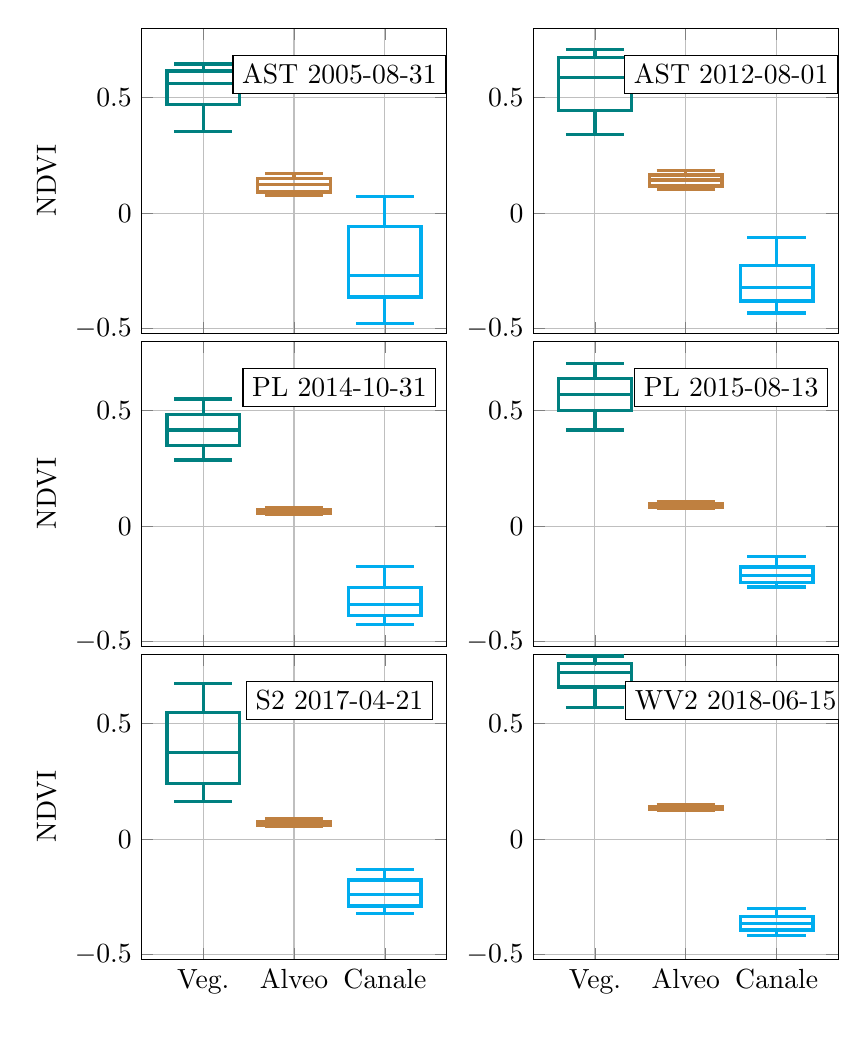
\begin{tikzpicture}
	\begin{groupplot}[
		group style = {
			group size = 2 by 3,
			ylabels at = edge left,
			x descriptions at = edge bottom,
			horizontal sep = 1.1cm,
			vertical sep = 0.1cm,
		},
		width = 0.45\textwidth,
		height = 0.45\textwidth,
		ylabel = NDVI,
		boxplot/draw direction = y,
		xtick = {1,2,3},
		xticklabels = {Veg., Alveo, Canale},
		ymax = 0.8,
		ymin = -0.52,
		grid = major,
	]
	\nextgroupplot % ASTER 2005-08-31
		\addplot+ [ % vegetazione
			teal, very thick,
			boxplot prepared = {
				lower whisker = 0.353656,
				lower quartile = 0.470411,
				median = 0.560063,
				upper quartile = 0.614701,
				upper whisker = 0.644957,
				},
        	]
        	coordinates {};
		\addplot+ [ % alveo attivo
			brown, very thick,
			boxplot prepared = {
				lower whisker = 0.077472,
				lower quartile = 0.091653,
				median = 0.122488,
				upper quartile = 0.149573,
				upper whisker = 0.171459,
				},
        	]
        	coordinates {};
		\addplot+ [ % canale
			cyan, very thick,
			boxplot prepared = {
				lower whisker = -0.477885,
				lower quartile = -0.362798,
				median = -0.269905,
				upper quartile = -0.058787,
				upper whisker = 0.072414,
				},
        	]
        	coordinates {};
        \node [fill = white, draw = black, anchor = center] 
        	at (2.5,0.6) {AST 2005-08-31};
	%------------------------------------------------------
	\nextgroupplot % ASTER 2012-08-01
		\addplot+ [ % vegetazione
			teal, very thick,
			boxplot prepared = {
				lower whisker = 0.341613,
				lower quartile = 0.444200,
				median = 0.586294,
				upper quartile = 0.672889,
				upper whisker = 0.709027,
				},
        	]
        	coordinates {};
		\addplot+ [ % alveo attivo
			brown, very thick,
			boxplot prepared = {
				lower whisker = 0.10506,
				lower quartile = 0.117969,
				median = 0.143631,
				upper quartile = 0.16549,
				upper whisker = 0.184871,
				},
        	]
        	coordinates {};
		\addplot+ [ % canale
			cyan, very thick,
			boxplot prepared = {
				lower whisker = -0.432201,
				lower quartile = -0.379825,
				median = -0.322239,
				upper quartile = -0.226459,
				upper whisker = -0.103914,
				},
        	]
        	coordinates {};
        \node [fill = white, draw = black, anchor = center] 
        	at (2.5,0.6) {AST 2012-08-01};
	%------------------------------------------------------
	\nextgroupplot % Pleiades 2014-10-31
		\addplot+ [ % vegetazione
			teal, very thick,
			boxplot prepared = {
				lower whisker = 0.286467,
				lower quartile = 0.350238,
				median = 0.415502,
				upper quartile = 0.483495,
				upper whisker = 0.549505,
				},
        	]
        	coordinates {};
		\addplot+ [ % alveo attivo
			brown, very thick,
			boxplot prepared = {
				lower whisker = 0.049796,
				lower quartile = 0.055794,
				median = 0.063049,
				upper quartile = 0.07173,
				upper whisker = 0.081427,
				},
        	]
        	coordinates {};
		\addplot+ [ % canale
			cyan, very thick,
			boxplot prepared = {
				lower whisker = -0.426415,
				lower quartile = -0.387978,
				median = -0.338308,
				upper quartile = -0.266515,
				upper whisker = -0.175373,
				},
        	]
        	coordinates {};
        \node [fill = white, draw = black, anchor = center] 
        	at (2.5,0.6) {PL 2014-10-31};
	%------------------------------------------------------
	\nextgroupplot % Pleiades 2015-08-13
		\addplot+ [ % vegetazione
			teal, very thick,
			boxplot prepared = {
				lower whisker = 0.415693,
				lower quartile = 0.5,
				median = 0.570359,
				upper quartile = 0.638507,
				upper whisker = 0.704044		
,
				},
        	]
        	coordinates {};
		\addplot+ [ % alveo attivo
			brown, very thick,
			boxplot prepared = {
				lower whisker = 0.075052,
				lower quartile = 0.080858,
				median = 0.087921,
				upper quartile = 0.096031,
				upper whisker = 0.106198,
				},
        	]
        	coordinates {};
		\addplot+ [ % canale
			cyan, very thick,
			boxplot prepared = {
				lower whisker = -0.262599,
				lower quartile = -0.244228,
				median = -0.214393,
				upper quartile = -0.176471,
				upper whisker = -0.132762,
				},
        	]
        	coordinates {};
        \node [fill = white, draw = black, anchor = center] 
        	at (2.5,0.6) {PL 2015-08-13};
	%------------------------------------------------------
	\nextgroupplot % Sentinel2 2017-04-21
		\addplot+ [ % vegetazione
			teal, very thick,
			boxplot prepared = {
				lower whisker = 0.163722,
				lower quartile = 0.241916,
				median = 0.374344,
				upper quartile = 0.548241,
				upper whisker = 0.672782,
				},
        	]
        	coordinates {};
		\addplot+ [ % alveo attivo
			brown, very thick,
			boxplot prepared = {
				lower whisker = 0.056176,
				lower quartile = 0.061278,
				median = 0.067681,
				upper quartile = 0.076396,
				upper whisker = 0.089304,
				},
        	]
        	coordinates {};
		\addplot+ [ % canale
			cyan, very thick,
			boxplot prepared = {
				lower whisker = -0.322237,
				lower quartile = -0.288822,
				median = -0.239533,
				upper quartile = -0.177094,
				upper whisker = -0.131119,
				},
        	]
        	coordinates {};
        \node [fill = white, draw = black, anchor = center] 
        	at (2.5,0.6) {S2 2017-04-21};
	%------------------------------------------------------
	\nextgroupplot % WorldView2 2018-06-15
		\addplot+ [ % vegetazione
			teal, very thick,
			boxplot prepared = {
				lower whisker = 0.569665,
				lower quartile = 0.657917,
				median = 0.719523,
				upper quartile = 0.759148,
				upper whisker = 0.791594,
				},
        	]
        	coordinates {};
		\addplot+ [ % alveo attivo
			brown, very thick,
			boxplot prepared = {
				lower whisker = 0.126214,
				lower quartile = 0.129661,
				median = 0.13373,
				upper quartile = 0.138542,
				upper whisker = 0.149326,
				},
        	]
        	coordinates {};
		\addplot+ [ % canale
			cyan, very thick,
			boxplot prepared = {
				lower whisker = -0.416974,
				lower quartile = -0.392405,
				median = -0.365385,
				upper quartile = -0.335135,
				upper whisker = -0.29979,
				},
        	]
        	coordinates {};
        \node [fill = white, draw = black, anchor = center] 
        	at (2.55,0.6) {WV2 2018-06-15};
	\end{groupplot}
\end{tikzpicture}

		\caption[boxplot dell'NDVI nelle aree campione in quattro immagini satellitari]{boxplot dell'NDVI nelle aree campione in quattro immagini satellitari; i baffi indicano il 10mo e il 90mo percentile, gli estremi della scatola rappresentano il 25mo e il 75mo percentile, la linea nella scatola è la mediana.}
		\label{graph:percentili}
	\end{figure}
	%
	%
	\item[Soglie NDVI] 
	Da tali grafici sono state ottenute delle soglie di NDVI per classificare le immagini satellitari (\vref{tab:ndvi-soglia}); per l'immagine \WV{} la soglia che distingue vegetazione da alveo attivo è maggiore. Le soglie sono in accordo con quanto riportato in letteratura \squarecite{Bertoldi:2011-ASTER}.
	%
	\begin{table}[ht]
		\centering
		\begin{tabular}{
			c 
			S[table-format=1.1]@{\,}
			c@{\,}
			c@{\,}
			c@{\,}
			S[table-format=1.1]
			S[table-format=1.1]@{\,}
			c@{\,}
			c@{\,}
			c@{\,}
			S[table-format=1.1]
			}
			\toprule
			&	\multicolumn{5}{c}{\textbf{Soglie AST PL S2}}	&	\multicolumn{5}{c}{\textbf{Soglie WV2}}	\\
			\midrule
			Vegetazione		&	0.2	&	$\leq$	&	NDVI	&			&		& 	0.3	&	$\leq$	&	NDVI	&			& 	\\
			Alveo attivo	&	0.0	&	$\leq$	&	NDVI	&	$<$		&	0.2	&	0.0	&	$\leq$	&	NDVI	&	$<$		&	0.3\\
			Canale			&		&			&	NDVI	&	$<$		&	0.0	&		&			&	NDVI	&	$<$		&	0.0\\
			\bottomrule
		\end{tabular}
		\caption[soglie NDVI]{soglie di NDVI per la classificazione delle immagini satellitari.}
		\label{tab:ndvi-soglia}
	\end{table}
	%
	%
	\item[Divisione in 23 tratti]
	La maschera di calcolo è stata suddivisa manualmente in 23~tratti con 22~sezioni al fine di avere un maggior dettaglio spaziale delle dinamiche di vegetazione (\vref{fig:23-tratti}). 
	Questi tratti sono stati selezionati in modo da possedere caratteristiche omogenee per portata e crescita della vegetazione; 
	pertanto confluenze di immissari, bruschi restringimenti o allargamenti, inizio di pronunciato \emph{upwelling} o \emph{downwelling} ed evidenti cambiamenti di morfologia fluviale sono stati gli elementi per individuare le 22~sezioni che determinano i 23~tratti.
	%
	\begin{figure}
		\centering
		\includegraphics[width=.8\textwidth]{files/tutti_23_tratti.jpeg}
		\caption[immagine con la maschera suddivisa in 23 tratti]{immagine con la maschera suddivisa in 23 tratti; la sezione di monte del tratto~1 corrisponde a Tolmezzo, la sezione di valle del tratto~23 corrisponde al ponte di Madrisio.}
		\label{fig:23-tratti}
	\end{figure}
	%
	%
	\item[isole e \emph{Floodplain}]
	Tramite una procedura semi-automatica e con il supporto di Google Earth, la classe della vegetazione è stata suddivisa in \emph{floodplain} e isole. 
	Tale procedura si basa sul fatto che la maschera computazionale comprende parte della piana alluvionale e che le isole sono completamente circondate dalla ghiaia dell'alveo durante periodi di magra.
	\\
	Successivamente, un controllo visivo del risultato e una correzione manuale di alcune celle hanno permesso sia di distinguere correttamente le isole, sia di evitare che isole molto prossime alla \emph{floodplain} ne fossero considerate parte; la classe delle celle corrette è stata aggiunta alla classificazione.
	%
	%
	\item[Nuvole e nodata] Alcune immagini presentano una lieve copertura nuvolosa che si estende nella maschera; queste zone sono state manualmente delimitate poiché presentano valori NDVI alterati.
	\\
	Altre immagini hanno un'estensione limitata rispetto alla maschera; questo porta ad avere aree prive di dati (\texttt{nodata}).
	\\
	Alla classificazione sono state aggiunte la classe delle nuvole e dei \texttt{nodata}.
	%
	%
	\item[Classificazione finale dei tratti] La \vref{tab:class_tratti} mostra le classi in cui è stato classificato ognuno dei 23~tratti; la \vref{fig:class_is_fl} ne mostra un esempio.
	%
	\begin{table}[ht]
		\centering
		\begin{tabular}{
			c 
			c
			}
			\toprule
			\textbf{Macroclasse}	&	\textbf{Classe}	\\
			\midrule
			Vegetazione		&	Isola	\\
							&	Floodplain	\\
			Alveo attivo	&	Cella corretta	\\
							&	Ghiaia	\\
							&	Canale	\\
			Altro			&	Nuvola	\\
							&	Nodata	\\
			\bottomrule
		\end{tabular}
		\caption[classificazione dell'area dei tratti]{classificazione finale dell'area di ogni tratto all'interno della maschera computazionale.}
		\label{tab:class_tratti}
	\end{table}
	%
	\begin{figure}[ht]
		\centering
		\includegraphics[width=.8\textwidth]{files/esempio_class_is_fl.jpeg}
		\caption[esempio della classificazione dell'area dei tratti]{esempio della classificazione dell'area dei tratti; la zona raffigurata si colloca a ridosso del ponte autostradale a valle di Braulins.}
		\label{fig:class_is_fl}
	\end{figure}
	%

Al fine di validare la precedente procedura di controllo e correzione della distinzione isole - \emph{floodplain}, si è osservato per ogni tratto l'andamento temporale della larghezza media~$B$, esprimibile semplicemente come il rapporto dell'area dell'alveo di ogni tratto (somma dell'alveo attivo e delle isole) per la sua lunghezza seguendo la corrente:
	%
	\begin{equation}
		\label{eq:larghezza-tratto}
		B = \frac{\text{Area alveo}}{Lunghezza} 
		\quad .
	\end{equation}
	% 
	Si è verificato che la larghezza~$B$ rimanesse costante nel tempo, indice di una corretta classificazione tra isole e \emph{floodplain}. 
	La~$B$ non rimane costante solo nel caso di distacco di isole o di fusione di isole nella piana. 
	\\
	La \vref{fig:b-media-7-e-15} mostra l'andamento temporale della~$B$ dei tratti~7 e~15: nel primo tratto, in cui non si osserva alcuna variazione sensibile dell'alveo, la~$B$ oscilla solo di qualche decina di metri; nel secondo si assiste alla progressiva fusione di una grande isola nella \emph{floodplain}, e questo lo si vede proprio nella diminuzione della~$B$. Ciò che conta non è quanto è largo l'alveo, ma quanto cambia la larghezza.
	%
	\begin{figure}
		\centering
		\tikzsetnextfilename{larghezze_tr_7_tr_15}
\begin{tikzpicture}
	\begin{axis}[
		width = 0.6\textwidth,
		height = 0.5\textwidth,
		date coordinates in = x,
		date ZERO = 2000-01-01,
		xticklabel = {$\year$},
		xticklabel style = {
			rotate = 80,
			anchor = near xticklabel
		},
		xtick distance = 730,
		enlarge x limits = 0.05,
		enlarge y limits = 0.01,
		ylabel = {Larghezza media dell'alveo \si{[\m]}},
		grid = major,
		]        
		\addplot+[blue]
        	table [x = data, y = tr_15] {graphics/data/Larghezze_medie_alveo.txt};
        \addlegendentry{Tratto 15}
        
		\addplot+[orange]
        	table [x = data, y = tr_7] {graphics/data/Larghezze_medie_alveo.txt};
        \addlegendentry{Tratto 7}
	\end{axis}
\end{tikzpicture}

		\quad
		\includegraphics[width=0.3\textwidth]{files/fusione_isola_tr_15.jpeg}
		\caption[andamento temporale di $B$ per i tratti~7 e~15]{a sinistra si vede l'andamento nel tempo della larghezza media dei tratti~7 e~15; la $B$ del tratto~7 oscilla solamente di qualche decina di metri, mentre il tratto~15 riduce improvvisamente la sua $B$ a causa della fusione di una grande isola nella \emph{floodplain}, fenomeno mostrato a destra (A: 2003-11-29, B: 2005-08-30).}
		\label{fig:b-media-7-e-15}
	\end{figure}
	
\end{description}


\begin{comment}
%TODO tenere questa parte? forse la si può togliere
% e mostrare direttamente i risultati sul cambiamento
Con la riclassificazione delle immagini dell'NDVI rispetto alle soglie proposte è stato possibile ottenere la percentuale di alveo coperta da vegetazione per ogni anno. 
Si ricorda, grazie alla maschera applicata, tale copertura include sia isole vegetate sia la parte di piana alluvionale che nel periodo di studio ha esperito fenomeni di erosione della vegetazione e quindi espansione dell'alveo attivo.
Infine, per le immagini l'alveo parzialmente coperto da nuvole, la maschera è stata estesa per escludere tali zone coperte poiché queste presentano valori di NDVI non corretti.
\\
I risultati sono mostrati nel grafico in \vref{graph:class-sat-veg}.


\begin{figure}[ht]
	\centering
	\begin{tikzpicture}
	\begin{axis}[
		width = \textwidth,
		height = 0.5\textwidth,
		date coordinates in = x,
		date ZERO = 2000-01-01,
		xticklabel = {\year},
		xticklabel style = {
			rotate = 80,
			anchor = near xticklabel
		},
		axis y line* = right,
		%ymax = 70,
		%ymin = 0,
		ylabel = {Percentuale di vegetazione},
		grid = none,
		]
		\addplot+
        	[red, mark=+, ultra thick]
        	table [x=data, y=veg] {graphics/data/Class_sat_veg-H2O-ghiaia.txt};
	\end{axis}
	
	\begin{axis}[
		width = \textwidth,
		height = 0.5\textwidth,
		date coordinates in = x,
		date ZERO = 2000-01-01,
		xticklabel = {\year},
		xticklabel style = {
			rotate = 80,
			anchor = near xticklabel
		},
		axis y line* = left,
		axis x line = none,
		enlarge x limits = 0.05,
		enlarge y limits = 0.01,
		ymax = 3.7,
		ymin = 2,
		ylabel = {Livello idrometrico \si{[\m]}},
		grid = none,
		]
		\addplot+
        	[blue, no markers, ultra thin]
        	table [x=data, y=media-gg] {graphics/data/Dati_Villuzza.csv};
	\end{axis}
\end{tikzpicture}

	\caption[andamento dell'areale della vegetazione nelle isole  e nella floodplain]{andamento dell'areale della vegetazione nelle isole e nella floodplain (in rosso). I dati provengono dalla classificazione delle immagini satellitari (\AST{}, \Pl{}, \Se{} e \WV{}). In blu sono mostrati i livelli idrometrici medi giornalieri superiori a~\SI{2}{\m} registrati alla stazione di Villuzza.}
	\label{graph:class-sat-veg}
\end{figure}
% grafico piene 2m+ - %veg tratti (nuovo file comprensivo di tutti i tratti)
\end{comment}



\subsection{Risultati: evoluzione della larghezza}
Utilizzando le mappe di classificazione del terreno all'interno della maschera computazionale, si è ottenuta una larghezza media~$B$ secondo l'equazione~\eqref{eq:larghezza-tratto}.
%TODO \vref{eq:larghezza-tratto}. 
\\
Osservando la variazione temporale di~$B$ è possibile evincere delle traiettorie evolutive sia a livello di singolo tratto, sia a scala più ampia.
Inoltre, considerando la variazione spaziale (da monte verso valle) dell'areale delle isole, sono evidenti i pattern di \emph{upwelling} o \emph{downwelling} utilizzati durante la definizione dei 23~tratti.






\section{Cambiamento delle isole}
A partire dalle mappe di classificazione dell'alveo, sono state ottenute mappe sul cambiamento che le isole hanno, o non hanno, esperito: erosione, crescita, fusione nella \emph{floodplain} o permanenza (nessun cambiamento).
Il risultato sono i dati di partenza per ricercare relazioni con gli eventi di piena.
\\
A tal fine, ogni mappa è stata confrontata con quella temporalmente precedente.
\\
L'analisi si è focalizzata sulle isole, escludendo così la piana alluvionale.

\subsection{Metodi: ottenere il cambiamento}
\paragraph{Limitazioni} \label{par:camb-limiti}
Alcune mappe hanno una estensione limitata oppure presentano zone con copertura nuvolosa: ciò riduce il numero di confronti possibili per alcuni tratti. 
Dalle 23 immagini satellitari (si veda la \vref{tab:date-orto-sat}) si sono ottenute in media 16~immagini per tratto.

Inoltre, le immagini \AST{} non sono correttamente georeferenziate e non sono perfettamente sovrapponibili; l'entità di questo scostamento è dell'ordine di qualche cella.
Questo difetto è di grande importanza poiché per poter investigare l'evoluzione temporale delle isole occorre poter osservare nel tempo ogni cella; se questa si sposta da un'immagine alla successiva, il confronto non è più valido.
\\
La soluzione adottata è stata quella di traslare ogni mappa a nord, sud, est o ovest del numero di celle necessario per poterla sovrapporre alla mappa temporalmente precedente.
L'operazione è stata ripetuta per ogni confronto, per ogni tratto, ed è stata verificata visivamente.
Il massimo errore residuo è di 1~cella di scostamento in pochissime zone nei primi tratti (\numrange[range-phrase={ - }]{1}{4}); data la locale topografia montuosa si è preferito ridurre l'errore a tale entità e tenerlo sotto controllo piuttosto di distorcere la mappa con altre misure di georettifica.
\\
Le altre immagini sono invece correttamente georeferenziate.

Infine, per poter confrontare immagini a diversa dimensione di cella, come le \AST{} a~\SI{15}{\m} con le \Pl{} a~\SI{0.5}{\m}, è stato necessario ricampionare le immagini con la dimensione minore (ad esempio le \Pl{}) alla risoluzione di quelle a dimensione maggiore (le \AST{} o le \Se{}).
\\
Nel ricampionamento l'areale delle isole subisce un incremento o una riduzione, così come l'areale della ghiaia e delle altre classi in quanto nelle celle a dimensione maggiore sono presenti numerose celle a dimensione minore, ognuna con un valore diverso (\vref{fig:ricamp-explanation}).
%
\begin{figure}
	\centering
	\includegraphics[width=.9\textwidth]{files/ricamp_griglia.jpeg}
	\caption[celle a risoluzione diversa]{immagine \Pl{} 2015-08-13 a~\SI{0.5}{\m} sullo sfondo con la griglia a~\SI{15}{\m} in primo piano; si vede come diverse celle più piccole siano contenute in una singola cella maggiore.}
	\label{fig:ricamp-explanation}
\end{figure}
%
Nel ricampionamento si sceglie quale valore assegnare alla nuova cella più grande in base ai valori delle celle minori; nel presente lavoro si è scelto di assegnare un percentile.
La scelta del percentile è stata effettuata confrontando la radice quadrata della somma dei quadrati residui (RSQR):
%
\begin{equation}
	\label{eq:rad-som-quad-res}
	RSQR = \left\lbrace \sum_{n=1}^{cl} \left[\left( \frac{area_{\mathrm{orig,n}}}{area_{\mathrm{orig,tot}}} - \frac{area_{\mathrm{perc,n}}}{area_{\mathrm{perc,tot}}} \right)^2 \right] \right\rbrace ^ \frac{1}{2}	
\end{equation}
%
dove 
\begin{itemize}
	\item $cl$ è il numero di classi (\vref{tab:class_tratti});
	\item $n$ indica la $n$-esima classe;
	\item $area_{\mathrm{orig,n}}$ e $area_{\mathrm{perc,n}}$ sono rispettivamente l'area della $n$-esima classe nella mappa originale e in quella ricampionata ad un percentile;
	\item $area_{\mathrm{orig,tot}}$ e $area_{\mathrm{perc,tot}}$ sono rispettivamente l'area totale della mappa originale e in quella ricampionata ad un percentile. 
\end{itemize} 
%
Si è scelto di normalizzare l'area di ogni classe per l'area totale per lavorare con percentuali.
\\
Nei ricampionamenti da \SI{0.5}{\m} il $50_\mathrm{mo}$ percentile (mediana) è quello che mostra il minor RSQR ($<\SI{3}{\percent}$); in quelli da \SI{10}{\m} il $75_\mathrm{mo}$ percentile (terzo quartile) è il migliore ($RSQR<\SI{6}{\percent}$). Un esempio del risultato ottenuto è mostrato in \vref{fig:ricampionamento}.
%
\begin{figure}
	\centering
	\includegraphics[width=\textwidth]{files/ricamp_class_is_fl.jpeg}
	\caption[confronto originale - ricampionamento]{a sinistra l'immagine \WV{} originale, poco a valle dell'isola di Cornino; a destra la stessa immagine ricampionata distribuendo i valori con la mediana.}
	\label{fig:ricampionamento}
\end{figure} 
%


\paragraph{Confronti validi}
Dalle 23 immagini satellitari è stato possibile ottenere il numero di confronti mostrati in \vref{tab:confronti}. 
I confronti effettuati hanno la massima risoluzione temporale possibile, cioè per ogni tratto si sono confrontate le immagini valide temporalmente più vicine in modo da poter osservare gli effetti cumulati del minor numero possibile di eventi di piena.
%
\begin{table}
	\centering
	\begin{tabular}{
		S[table-format=2.0] 
		S[table-format=2.0]
		c 
		c}
		\toprule
		\textbf{Tratto}	&	\textbf{Confronti}	&	\textbf{Primo}		&	\textbf{Ultimo}	\\
						&	\textbf{validi}		&	\textbf{confronto}	&	\textbf{confronto}	\\
		\midrule
		1	&	13	&	2000-09-17/2003-06-22	&	2016-09-13/2017-04-21	\\
		2	&	13	&	2000-09-17/2001-06-17	&	2016-09-13/2017-04-21	\\
		3	&	16	&	2000-09-17/2001-06-17	&	2016-09-13/2017-04-21	\\
		4	&	16	&	2000-09-17/2001-06-17	&	2016-09-13/2017-04-21	\\
		5	&	16	&	2000-09-17/2001-06-20	&	2016-09-13/2017-04-21	\\
		6	&	18	&	2000-09-17/2001-06-17	&	2017-04-21/2018-06-15	\\
		7	&	18	&	2000-09-17/2001-06-17	&	2017-04-21/2018-06-15	\\
		8	&	19	&	2000-09-17/2001-06-17	&	2017-04-21/2018-06-15	\\
		9	&	18	&	2000-09-17/2002-05-18	&	2017-04-21/2018-06-15	\\
		10	&	18	&	2000-09-17/2002-05-18	&	2017-04-21/2018-06-15	\\
		11	&	18	&	2000-09-17/2002-05-18	&	2017-04-21/2018-06-15	\\
		12	&	18	&	2000-09-17/2002-05-18	&	2017-04-21/2018-06-15	\\
		13	&	18	&	2000-09-17/2002-05-18	&	2017-04-21/2018-06-15	\\
		14	&	21	&	2000-09-17/2002-05-18	&	2017-04-21/2018-06-15	\\
		15	&	16	&	2000-09-17/2002-06-12	&	2016-09-13/2017-04-21	\\
		16	&	16	&	2000-09-17/2002-06-12	&	2016-09-13/2017-04-21	\\
		17	&	16	&	2000-09-17/2002-06-12	&	2016-09-13/2017-04-21	\\
		18	&	16	&	2000-09-17/2002-06-12	&	2016-09-13/2017-04-21	\\
		19	&	13	&	2000-09-17/2002-06-12	&	2016-09-13/2017-04-39	\\
		20	&	13	&	2000-09-17/2002-06-12	&	2014-09-28/2015-09-11	\\
		21	&	13	&	2000-09-17/2002-06-12	&	2014-09-28/2015-09-11	\\
		22	&	13	&	2000-09-17/2002-06-12	&	2014-09-28/2015-09-11	\\
		23	&	12	&	2002-06-12/2003-06-22	&	2014-09-28/2015-09-11	\\
		\bottomrule
	\end{tabular}
	\caption[confronti effettuati]{confronti effettuati con le 23 immagini satellitari a disposizione per ottenere dati sul cambiamento delle isole.}
	\label{tab:confronti}
\end{table}
%

\paragraph{Classi del cambiamento}
In ogni confronto ci si è concentrati sul ciò che è successo alle isole, definendo quindi le seguenti 4~classi (si veda anche la \vref{tab:class_tratti}):
%
\begin{itemize}
	\item erosione (da isola ad alveo attivo);
	\item crescita (da alveo attivo ad isola);
	\item fusione nella \emph{floodplain} (da isola a \emph{floodplain});
	\item distaccamento dalla \emph{floodplain} (da \emph{floodplain} a isola);
	\item nessun cambiamento (da isola a isola).
\end{itemize}
%
Un esempio di questa classificazione è riportato nella \vref{fig:confr-class-is-fl}.
%
\begin{figure}
	\centering
	\includegraphics[width=.8\textwidth]{files/confr_class_is_fl.jpeg}
	\caption[esempio di mappa di cambiamento]{esempio di mappa di cambiamento ottenuta con il confronto tra le immagini \AST{} 2008-07-05 e 2010-09-29. Si possono osservare tutti i cambiamenti possibili; la prima classe serve solamente a visualizzare l'area della maschera computazionale. Il tratto mostrato è posto qualche \si{\kilo\m} a monte del ponte di Madrisio.}
	\label{fig:confr-class-is-fl}
\end{figure}
%


\subsection{Risultati: eventi eccezionali}
Dall'osservazione dell'idrogramma in \vref{graph:livelli-orto-sat} (riportato \vpageref{graph:tr-17-camb}) si può ipotizzare che le piene maggiori, come quelle avvenute verso la fine degli anni~2012 e~2014, siano quelle che abbiano asportato il maggior quantitativo di isole.
\\
I grafici in \vref{graph:tr-17-camb} mostrano alcuni risultati ottenuti dalle mappe di cambiamento per il tratto~17, posto nel tratto vallivo immediatamente a valle della confluenza con il torrente Cosa.
I dati sono rappresentati con due simboli: il pallino rappresenta la data finale di ogni confronto, mentre la croce indica la data iniziale; 
chiaramente il pallino di un confronto ha la stessa data della croce del confronto successivo. 
La croce serve solamente a sapere quanto dura ogni confronto; il pallino è il dato vero e proprio.
I dati sono normalizzati per l'areale delle isole nell'immagine \AST{} del 2000-09-17.
\\
Ciò che si vede è una spiccata crescita a cavallo degli anni~2006 e~2008, seguita da una erosione delle medesime proporzioni.
Dall'altra parte, nonostante la maggior intensità e durata le piene del 2012 e del~2014 hanno eroso meno di quanto ci si aspettava.
%
\begin{figure}
	\centering
	\begin{tikzpicture}
	\begin{axis}[
		width = \textwidth,
		date coordinates in = x,
		xticklabel = {\year-\month-\day},
		xticklabel style = {
			rotate = 90,
			anchor = near xticklabel
		},
		]
		\addplot table [x=data, y=media-gg] {graphics/data/Dati_Villuzza.csv};
	\end{axis}
\end{tikzpicture}
	\\
	\tikzsetnextfilename{tr_17_camb}
\begin{tikzpicture}
	\begin{groupplot}[
		group style = {
			group size = 2 by 1,
			ylabels at = edge left,
			x descriptions at = edge bottom,
			horizontal sep = 1cm,
			vertical sep = 0.1cm,
		},
		width = 0.5\textwidth,
		height = 0.5\textwidth,
		date ZERO = 2000-01-01,
		date coordinates in = x,
		xticklabel = {$\year$},
		xticklabel style = {
			rotate = 80,
			anchor = near xticklabel
		},
		xtick distance = 731,
		%ymax = 0.35,
		ylabel = {Cambiamento/Isole iniziali},
		grid = major,
		]
	\nextgroupplot % tr_17_accrescimento
		\addplot+
        	[only marks, blue]
        	table [
        		x=data_fine, 
        		y = alv->is,
        		] {graphics/data/tr_17_camb_eros_accr.txt};
		\addplot+
        	[only marks, mark=x, black]
        	table [
        		x=data_ini, 
        		y = alv->is,
        		] {graphics/data/tr_17_camb_eros_accr.txt};
        \node [fill = white, draw = black, anchor = south west] 
        	at (axis description cs: 0.05,0.8) {Accr.};
	\nextgroupplot % tr_17_erosione
		\addplot+
        	[only marks, blue]
        	table [
        		x=data_fine, 
        		y = is->alv,
        		] {graphics/data/tr_17_camb_eros_accr.txt};
		\addplot+
        	[only marks, mark=x, black]
        	table [
        		x=data_ini, 
        		y = is->alv,
        		] {graphics/data/tr_17_camb_eros_accr.txt};
        \node [fill = white, draw = black, anchor = south west] 
        	at (axis description cs: 0.05,0.8) {Eros.};
	\end{groupplot}
\end{tikzpicture}

	\caption[cambiamenti esperiti dalle isole nel tratto~17]{cambiamenti esperiti dalle isole nel tratto~17 rappresentati come percentuale rispetto all'areale delle isole nella prima immagine utile. 
	Si nota il dato relativo al confronto 2008-07-05/2010-09-29, particolarmente elevato e di pari entità tra crescita ed erosione.}
	\label{graph:tr-17-camb}
\end{figure}
%
Questa osservazione può trovare la seguente giustificazione: il periodo privo di piene con livello al disopra dei \SI{2}{\m} tra fine del 2004 e la fine del 2008 è stato favorevole per l'insediamento di nuova vegetazione;
le macchie vegetate sono diventate visibili da satellite solamente quando le piante hanno sviluppato una chioma sufficientemente ampia, cioè dopo qualche anno, nell'immagine del 2008-07-05;
questa più recente vegetazione si è espansa sulle barre e sulle forme morfologiche a quota minore rispetto alle isole più vecchie;
con questi fatti, la prima piena che è giunta ha facilmente portato via tutte queste isole giovani e basse.
\\
Occorre quindi ragionare non solo in termini di singoli eventi di piena, ma estendere le proprie considerazioni all'intero idrogramma, al periodo di tempo tra piene oltre un certo livello, alla loro frequenza, poiché sono questi i fattori che possono determinare le dinamiche delle isole.
Il periodo 2005-2008 privo di grandi piene può essere considerato un evento tanto importante quanto la piena lunga ed intensa del mese di Novembre, 2014.

%TODO c'è un trend: i tratti con upwelling sono quelli che si vegetano di più


Da queste osservazioni il passo successivo è naturale: trovare la composizione delle isole in termini di età e riflettere se è la vegetazione più giovane quella ad essere più facilmente erosa.




\section{Età della vegetazione nelle isole}
Utilizzando le mappe del cambiamento esperito dalle isole si possono ottenere mappe che indicano un'età approssimativa della vegetazione che compone queste isole. 
\\
L'ipotesi che si vuole verificare è che sia la vegetazione più giovane quella ad essere maggiormente erosa in quanto può essere divelta più facilmente.
Non si esclude tuttavia di osservare erosione anche di vegetazione matura poiché le isole poste in corrispondenza dell'estradosso di un canale curvo sono soggette a scavo laterale.

\subsection{Metodi: estendere i confronti e ottenere un'età}
\paragraph{Limiti}
Con le immagini satellitari utilizzate non è possibile distinguere i singoli alberi che compongono le isole; se con le immagini a miglior risoluzione si distinguono gli arbusti isolati, non si può certo ottenere una stima dell'età tanto precisa quanto quella fornita da un carotaggio del tronco.
In più, una cella è classificata come vegetazione solo quando le piante al suo interno presentano una chioma sufficientemente grande da occupare gran parte della cella; pertanto le immagini con celle di \SI{10}{\m} o addirittura \SI{15}{\m} non possono mostrare che grandi macchie di vegetazione.
Prima dei \SI{3}{\anni} una pianta di salice generalmente non ha fronde molto estese.
\\
Occorre poi tenere in conto che le piante crescono differentemente in base alle condizioni ambientali: periodi di stress idrico o termico rallentano la crescita, così come il parziale seppellimento con ghiaia dovuto ad eventi di piena; una falda non troppo profonda la cui altezza varia lentamente, terreno di granulometria sottile con sabbia e buone temperature sono invece fattori favorevoli alla crescita \squarecite{Gurnell:2001-island-formation}.

Si crede che ciò che possa accadere è che fino ad una certa età, circa \SI{3}{\anni}, la nuova vegetazione non sia visibile dal satellite. 

Le mappe del cambiamento sono state ottenute dalle mappe di classificazione; non essendo le seconde correttamente georeferenziate, neanche le prime lo sono. L'errore residuo nel processo di correzione è di 1~cella.

Infine, per poter confrontare nel corso degli anni ogni cella, le mappe del cambiamento sono state ricampionate alla risoluzione più bassa, corrispondente a celle di~\SI{15}{\m} di lato. Si è proceduto come mostrato nel paragrafo \ref{par:camb-limiti} ottenendo valori $RSQR < \SI{1.5}{\percent}$.
 

%TODO le piante crescono diversamente in base alle condizioni ambientali (cita articolo Gurnell?) → definire un'età in base al tempo di osservazione è un approccio limitato (qualche altro lavoro simile)

\paragraph{Obiettivo ed approccio} 
Date le precedenti premesse, bisogna riflettere su ciò che si vuole ottenere: dividere la vegetazione in classi di età.
Si vuole sapere quanta vegetazione giovane è stata erosa; non importa se questa ha esattamente \SI{3}{\anni} o \SI{4}{\anni}, l'importante è che sia grossomodo classificata come giovane.

Ogni mappa del cambiamento è formata dalle informazioni contenute in due mappe: quella più vecchia e quella più recente. La distanza temporale tra queste due mappe definisce il periodo di osservazione.
\\
Per la mappa del cambiamento più vecchia, l'età della vegetazione delle isole è stata arbitrariamente essere pari al periodo di osservazione, cui si sono aggiunti \SI{3}{\anni}.
\\
Per le mappe via via più recenti, l'età nelle celle delle isole che non sono cambiate è pari al periodo di osservazione sommato all'età precedente; per le celle si sono vegetate a partire dall'alveo l'età è pari al periodo di osservazione con l'aggiunta di \SI{3}{\anni}, ritenuto il periodo minimo affinché un insieme di piante diventi visibile per il satellite.

\medskip
L'approccio di definire un'età in base al periodo di osservazione è limitato, in particolare per le mappe più vecchie poiché non è possibile tener conto della vegetazione che era presente antecedentemente alla prima immagine valida;
si ritiene che a partire dalla $4^a$ o $5^a$ mappa di età il metodo inizi ad essere affidabile (generalmente quindi dalla mappa di età del 2007-09-21).
Per gli scopi della ricerca questo approccio risulta essere sufficiente.

\paragraph{Validazione}
Il CSM (\emph{Canopy Surface Model}) è il modello digitale della copertura arborea; similmente al DEM, mostra delle quote; queste sono tuttavia riferite all'altezza della vegetazione sopra il terreno.
\\
È generalmente sensato affermare che piante più mature abbiano un'altezza maggiore di piante giovani.
Quindi si sono utilizzate le informazioni del CSM relativo alla ortofoto del 2013-10-22 per verificare che nelle celle della mappa di età della vegetazione del 2013-09-05 l'altezza fosse all'incirca proporzionale all'età.
%TODO grafico con i quantili

\subsection{Risultati: un trend per la vegetazione erosa}
I grafici in \vref{graph:distr-eta} mostrano la distribuzione di età della vegetazione nelle isole in termini di areale occupato; per gli scopi del lavoro ci si limita a definire 3~classi di vegetazione:
%
\begin{itemize}
	\item giovane, con meno di \SI{5}{\anni};
	\item intermedia, con età compresa tra \SIrange[range-phrase={ e }]{5}{10}{\anni};
	\item matura, con più di \SI{10}{\anni}.
\end{itemize}

%TODO da migliorare (togliere la descrizione all'asse y?)
%
\begin{figure}
	\centering
	\begin{tikzpicture}
	\begin{groupplot}[
		group style = {
			group size = 1 by 3,
			ylabels at = edge left,
			x descriptions at = edge bottom,
			xticklabels at = all,
			horizontal sep = 1.1cm,
			vertical sep = 1cm,
		},
		width = \textwidth,
		%height = 0.6\textwidth,
		xbar stacked,
		%bar width = 5pt,
		%enlarge x limits = 0.05,
		%enlarge y limits = 0.01,
		xmin = 0,
		scaled x ticks = false,
		xtick distance = 1e5,
		xlabel = {Area occupata \si{[\m\tothe{2}]}},
		ylabel = {Mappa di età},
		grid = major,
		]
		\nextgroupplot [% tratto_8
			height = 0.45\textwidth,
			legend style = {
				at = {(0.5,1.05)},
				legend columns = 3,
				anchor = south
			}, 
			legend entries = {giovane, intermedia, matura},
			symbolic y coords = {
				2008-07-05, 2009-07-08, 
				2012-08-01, 2013-09-05,  
				2017-04-21, 2018-06-15
			},
			ytick = data,]
			\addplot
		       	table [y=data, x=giovane] {graphics/data/tr_8_eta.txt};
			\addplot
		       	table [y=data, x=intermedia] {graphics/data/tr_8_eta.txt};
			\addplot
		       	table [y=data, x=matura] {graphics/data/tr_8_eta.txt};
        	\node [fill = white, draw = black, anchor = north east] 
        		at (axis description cs: 1,1) {Tratto 8};
		\nextgroupplot [% tratto_11
			height = 0.3\textwidth,
			symbolic y coords = {
				2008-07-05, 2009-07-08, 
				2014-10-31, 2015-08-13, 
			},
			ytick = data,
		]
			\addplot
		       	table [y=data, x=giovane] {graphics/data/tr_11_eta.txt};
			\addplot
		       	table [y=data, x=intermedia] {graphics/data/tr_11_eta.txt};
			\addplot
		       	table [y=data, x=matura] {graphics/data/tr_11_eta.txt};
        	\node [fill = white, draw = black, anchor = north east] 
        		at (axis description cs: 1,1) {Tratto 11};
		\nextgroupplot [% tratto_17
			height = 0.45\textwidth,
			symbolic y coords = {
				2008-07-05, 2010-09-29,
				2012-08-01, 2013-09-05, 
				2014-09-08, 2015-09-11,
			},
			ytick = data,
		]
			\addplot
		       	table [y=data, x=giovane] {graphics/data/tr_17_eta.txt};
			\addplot
		       	table [y=data, x=intermedia] {graphics/data/tr_17_eta.txt};
			\addplot
		       	table [y=data, x=matura] {graphics/data/tr_17_eta.txt};
        	\node [fill = white, draw = black, anchor = north east] 
        		at (axis description cs: 1,1) {Tratto 17};
	\end{groupplot}
\end{tikzpicture}




	\caption[areale delle classi d'età per i tratti~8, 11 e~17]{areale delle tre classi di età per alcune immagini dei tratti~8, 11 e~17.}% \numlist[list-final-separator={ e }]{8;11;17}.}
	\label{graph:distr-eta}
\end{figure}
%

Focalizzandosi sugli eventi di piena della fine del~2008 e del~2012, si vede chiaramente come l'areale della vegetazione giovane sia fortemente diminuito dalle immagini antecedenti le piene alle immagini successive (tratti \numrange[range-phrase={ e }]{11}{17});
sia in termini relativi che in termini assoluti, la vegetazione giovane è quella che è prevalentemente portata via dalle piene, quando è presente;
in seguito alle due piene considerate si osserva inoltre una diminuzione dell'area occupata dalle isole.
Si tenga comunque in conto che parte della vegetazione non erosa invecchia e può passare da una classe a quella successiva; questo fenomeno non è tuttavia quello predominante durante le piene del~2008 e del~2012 per evidenza.
\\
Con il confronto tra anni in cui non c'è stata una forte espansione delle isole ma in cui ci sono stati particolari eventi, come tra il \numrange[range-phrase={ e il }]{2014}{2015} o tra il \numrange[range-phrase={ e il }]{2017}{2018}, non si nota un cambiamento particolare nella distribuzione d'età.
%Anzi, nell'undicesimo tratto, dove sono presenti grandi isole, la piena ne ha probabilmente asportato alcune con età intermedia

% magari secondo grafico con stesso tratto, stesse immagini ma solo vegetazione erosa


















%----------------------------------------------------------




%----------------------------------------------------------
% aggiunge tutte le voci del glossario
\glsaddall
%----------------------------------------------------------
%**********************************************************
%**********************************************************
\backmatter

% glossario
\manualmark
\markboth{\spacedlowsmallcaps{\glossaryname}}%
{\spacedlowsmallcaps{\glossaryname}}
\phantomsection
\pagestyle{scrheadings}
\addcontentsline{toc}{chapter}{\tocEntry{\glossaryname}}
\printglossaries

% bibliografia
\printbibliography

\end{document}
